\documentclass[xcolor={dvipsnames,table}]{beamer}
\mode<presentation>{\usetheme{Warsaw}\usecolortheme{crane}}
\usepackage{centernot}
\usepackage{graphicx}
\usepackage{geometry}
\usepackage{tikz}
\usetikzlibrary{shadows}

\usefonttheme{serif}
\usepackage[utf8]{inputenc}
\usepackage[english]{babel}
\usepackage{lmodern}
\usepackage[T1]{fontenc}
\usepackage[babel=true]{microtype}

\title{UNIX Weapons School---The x86}
\date{}
\author{Nick Black for the\\
Georgia Institute of Technology
}

\begin{document}

\begin{frame}
\titlepage
\begin{center}
\includegraphics[scale=0.33]{images/uws.png}\\
\vspace{.1in}
\tiny{copyright \copyright\ 2013}\\
\includegraphics[scale=.25]{images/cc-logo.pdf}

\includegraphics[scale=.25]{images/cc-new.pdf}

\includegraphics[scale=.25]{images/cc-share.pdf}\\
\tiny{creative commons 3.0 share-alike attribution license}
\end{center}
\end{frame}

\begin{frame}{Why study the x86?}
\begin{itemize}
\item Used in a majority of servers, workstations, and laptops
\item Receives the most focus in the kernel/toolchain
\item Very complex processor, thus large optimization space
\item Excellent documentation and literature
\item Fascinating and revealing history
\end{itemize}
\end{frame}

\begin{frame}[t]{16-bit era (IBM PC, MS-DOS, PDP-11, Alto)}
\begin{block}{8086/80186 (Intel, NEC, AMD, Fujitsu, OKI, Kvazar-Mikro\ldots)}
\begin{itemize}
\item Real mode (x86-16 ISA) \hfill \includegraphics[height=11pt]{images/kp1810trans.jpg}
\item 1MB RAM in 16 64K segments
\item 8086-2 ISA on 80186
{\footnotesize
(\tt{ENTER}/\tt{LEAVE}, \tt{PUSHA}/\tt{POPA}, \tt{INS}/\tt{OUTS})
}
\end{itemize}
\end{block}
\begin{block}{80286 (Intel, IBM, AMD, Fujitsu\ldots)}
\begin{columns}
\column{3.4in}
\begin{itemize}
\item Protected mode w/ MMU
\item 16MB RAM with privilege levels on segments
\end{itemize}
\column{.5in}
%\includegraphics[width=.5in]{images/286.png}
\end{columns}
\end{block}
\vfill
\begin{center}
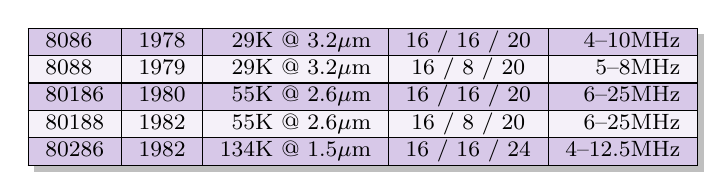
\begin{tikzpicture}
\node[drop shadow,fill=white,inner sep=0pt]
{\rowcolors{1}{RoyalPurple!20}{RoyalPurple!5}
{\footnotesize
\begin{tabular}{|l|r|r|c|r|}
\hline
8086 & 1978 & 29K @ 3.2$\mu$m & 16 / 16 / 20 & 4--10MHz \\
\hline
8088 & 1979 & 29K @ 3.2$\mu$m & 16 / 8 / 20 & 5--8MHz \\
\hline
80186 & 1980 & 55K @ 2.6$\mu$m & 16 / 16 / 20 & 6--25MHz \\
\hline
80188 & 1982 & 55K @ 2.6$\mu$m & 16 / 8 / 20 & 6--25MHz \\
\hline
80286 & 1982 & 134K @ 1.5$\mu$m & 16 / 16 / 24 & 4--12.5MHz \\
\hline
\end{tabular}%
}
};
\end{tikzpicture}
\end{center}
\end{frame}


\end{document}
